% ============================================================
%  LIVRABLE COMPLET — Supervision du portefeuille de projets IT
%  Time'Eats — Cellule PMO — CESI MAALSI Semestre 2
% ============================================================
\documentclass[11pt,a4paper,oneside]{report}

\PassOptionsToPackage{backend=bibtex}{biblatex}
\usepackage{style/consulting}
\usepackage{graphicx}
\graphicspath{{img/}}
\addbibresource{references.bib}

% Surcharge hyperref pour ce document
\hypersetup{
  pdftitle={Time'Eats — Supervision du portefeuille de projets IT},
  pdfauthor={Cellule PMO — CESI MAALSI},
}

% Surcharge en-tête
\pagestyle{fancy}
\fancyhf{}
\renewcommand{\headrulewidth}{0pt}
\fancyhead[L]{%
  \begin{tikzpicture}[remember picture, overlay]
    \draw[cnNavy, line width=0.5pt] (0,0) -- (\textwidth,0);
  \end{tikzpicture}%
  \vspace{2pt}\small\textcolor{cnSlate}{Time'Eats \textbf{·} Supervision du portefeuille de projets IT — PMO}%
}
\fancyhead[R]{\small\textcolor{cnSlate}{\thepage}}
\fancyfoot[C]{\tiny\textcolor{cnSlate}{Document confidentiel — Cellule PMO — CESI MAALSI 2026}}

% Commandes RAG
\newcommand{\ragV}{\cellcolor{cnGreen!20}\textbf{\textcolor{cnGreen}{Vert}}}
\newcommand{\ragA}{\cellcolor{cnOrange!20}\textbf{\textcolor{cnOrange}{Ambre}}}
\newcommand{\ragR}{\cellcolor{cnRed!20}\textbf{\textcolor{cnRed}{Rouge}}}

\begin{document}
\small

% ── Page de garde ────────────────────────────────────────────
\begin{titlepage}
  \pagecolor{cnNavy}
  \color{white}
  \vspace*{2.5cm}
  \begin{center}
    {\Huge\bfseries Time'Eats}\\[0.5cm]
    {\normalsize\textcolor{cnSlate} Cellule PMO — Direction des Systèmes d'Information}\\[2cm]
    \textcolor{cnOrange}{\rule{12cm}{1.5pt}}\\[1cm]
    {\LARGE\bfseries Supervision du portefeuille\\[0.3cm]de projets IT}\\[0.8cm]
    {\large Professionnalisation de la cellule PMO}\\[1cm]
    \textcolor{cnOrange}{\rule{12cm}{1.5pt}}\\[2cm]
    {\normalsize Projet Collaboratif — CESI MAALSI — Semestre 2}\\[0.4cm]
    {\normalsize Avril 2026}
  \end{center}
  \vfill
  \begin{center}
    \small\textcolor{cnSlate}{Budget portefeuille : 1\,700~K€ \quad|\quad 11 projets \quad|\quad DSI : 21 personnes}
  \end{center}
\end{titlepage}
\nopagecolor

\tableofcontents
\newpage

% ── Introduction ─────────────────────────────────────────────
\chapter*{Introduction}
\addcontentsline{toc}{chapter}{Introduction}

Time'Eats est une entreprise spécialisée en vente de nourriture préparée et livraison à domicile, basée à Rennes. Dans le cadre de son développement national, sa DSI de \textbf{21 personnes} doit piloter simultanément \textbf{11 projets IT} pour un budget total de \textbf{1\,700~K€}, avec un fort recours aux ESN.

\begin{finding}
Ce portefeuille est sous haute tension : une DSI de 21 personnes absorbe 11 projets majeurs avec des dépendances critiques, des échéances serrées et un budget global à maîtriser. Une méthodologie unique (tout Agile ou tout Cycle en V) ne peut suffire. La réponse est une \textbf{approche PMO hybride}, pragmatique et capacitaire.
\end{finding}

Ce document est structuré en trois parties correspondant aux axes d'évaluation :
\begin{enumerate}
  \item \textbf{Portefeuille de projets} — méthodologie, référentiel documentaire et tableau de bord de supervision
  \item \textbf{Gestion du projet CRM} — plan de management et tableau de bord de pilotage
  \item \textbf{Clôture et capitalisation} — documents contractuels, PV de recette et amélioration continue
\end{enumerate}

\begin{reco}
Les tableaux de bord de supervision (§1.3) et de pilotage CRM (§2.2) présentés dans ce livrable ont été \textbf{implémentés sous forme d'application web interactive} : le \textbf{Cockpit DSI Time'Eats}, développé en Node.js/Express. Ce cockpit constitue la \textit{source de vérité unique} du PMO conformément au Pilier 4 (§1.1). L'application est accessible en interne sur \texttt{http://localhost:3001}.
\end{reco}

\newpage

% ============================================================
% CHAPITRE 1 — PORTEFEUILLE DE PROJETS
% ============================================================
\chapter{Portefeuille de projets}

% ────────────────────────────────────────────────────────────
\section{Enjeux et objectifs généraux du portefeuille}

\begin{finding}
Time'Eats se trouve à un \textbf{tournant stratégique majeur} : l'entreprise doit simultanément consolider son socle technique, accélérer sa croissance nationale et professionnaliser sa DSI — le tout avec \textbf{21 personnes} et un budget de \textbf{1\,700~K€}. Le portefeuille de 11 projets n'est pas un catalogue de chantiers : c'est le \textbf{programme de transformation de l'entreprise pour les 12 prochains mois}. Sans cadre PMO structuré, ce volume de projets simultanés conduit inévitablement à des dérives budgétaires, des conflits de ressources et une perte de valeur livrée.
\end{finding}

\subsection{Enjeux du portefeuille}

\vspace{4pt}
\begin{center}
\renewcommand{\arraystretch}{1.6}
\begin{tabularx}{\textwidth}{C{2.5cm} L{5.5cm} L{6cm}}
\toprule
\rowcolor{cnNavy}
\th{Dimension} & \th{Enjeu identifié} & \th{Conséquence si non adressé} \\
\midrule
\textbf{Stratégique} & Aligner les 11 projets IT sur les priorités business de Time'Eats (croissance nationale, relation client, compétitivité) & Investissement IT déconnecté du terrain — ROI non perçu par la direction \\
\rowcolor{cnIce}
\textbf{Financier} & Maîtriser un budget global de 1\,700~K€ réparti sur des prestataires multiples, des modes contractuels variés et 12 mois d'exécution & Dépassements en cascade — arbitrages budgétaires brutaux en cours d'année \\
\textbf{Capacitaire} & Absorber 11 projets Build simultanés sans dégrader le Run (MCO), avec une DSI de 21 personnes dont 5 chefs de projet & Épuisement des équipes, glissement des délais, qualité sacrifiée \\
\rowcolor{cnIce}
\textbf{Opérationnel} & Gérer les dépendances inter-projets (Office~365 bloquant 3 projets majeurs) et les risques de propagation des retards & Effet domino sur CRM, Refonte Web et Apps mobiles \\
\textbf{Humain} & Piloter les ESN (contrats, livrables, satisfaction) tout en développant les compétences internes & Dépendance excessive aux prestataires, perte de souveraineté technique \\
\rowcolor{cnIce}
\textbf{Gouvernance} & Professionnaliser la cellule PMO pour produire une vision consolidée fiable en temps réel & Décisions prises sur des données obsolètes ou incomplètes \\
\bottomrule
\end{tabularx}
\end{center}

\subsection{Objectifs généraux du portefeuille}

Ces objectifs sont \textbf{mesurables et suivis} via le Cockpit DSI (§1.3). Ils constituent le cadre de succès du portefeuille que le PMO présente au Comité Stratégique mensuel.

\vspace{4pt}
\begin{center}
\renewcommand{\arraystretch}{1.6}
\begin{tabularx}{\textwidth}{C{0.4cm} L{5.5cm} C{2.5cm} C{2.5cm} L{2.5cm}}
\toprule
\rowcolor{cnNavy}
\th{\#} & \th{Objectif} & \th{Indicateur associé} & \th{Cible} & \th{Horizon} \\
\midrule
O1 & Livrer \textbf{100\,\%} des projets critiques (score $\geq 3{,}50$) dans le périmètre validé & Taux de respect du périmètre & 100\,\% & Déc. N \\
\rowcolor{cnIce}
O2 & Maîtriser le budget total du portefeuille à \textbf{$\pm$5\,\%} du prévisionnel & Taux de dépassement budgétaire & $\leq 5\,\%$ & Déc. N \\
O3 & Respecter les jalons critiques du portefeuille (démarrage, go-live) & \% jalons respectés & $\geq 80\,\%$ & Continu \\
\rowcolor{cnIce}
O4 & Garantir la \textbf{continuité de service} (Run) pendant la phase Build & Uptime moyen des 9 serveurs & $\geq 99\,\%$ & Mensuel \\
O5 & Résoudre les incidents P1 en moins de 5 jours ouvrés & Délai moyen résolution P1 & $\leq 5\,j$ & Continu \\
\rowcolor{cnIce}
O6 & Professionnaliser le PMO via un référentiel documentaire appliqué sur 100\,\% des projets & Taux de réutilisation des templates & $\geq 60\,\%$ & Juin N \\
O7 & Identifier \textbf{en amont} les risques majeurs (avant impact) & \% risques identifiés avant occurrence & $\geq 70\,\%$ & Continu \\
\bottomrule
\end{tabularx}
\end{center}

\begin{alert}
\textbf{Hiérarchisation des objectifs :} O4 (continuité de service) et O5 (incidents P1) sont non négociables — un incident P1 non résolu sous 5 jours impacte directement les revenus de Time'Eats (plateforme de livraison). Les objectifs O1 à O3 sont le cœur de la mission PMO.
\end{alert}

\newpage
% ────────────────────────────────────────────────────────────
\section{Méthodologie PMO Hybride}

\begin{decision}
Adopter une \textbf{méthodologie PMO Hybride à 4 piliers}, axée sur le pragmatisme et la gestion stricte de la capacité. Elle distingue les projets par nature et impose un rythme de gouvernance commun à l'ensemble du portefeuille.
\end{decision}

\subsection{Pilier 1 — Gouvernance par les rituels (tempo du PMO)}

Le PMO doit dicter le \textbf{rythme de pilotage} pour éviter la dispersion des ressources internes sur 11 fronts simultanés.

\vspace{4pt}
\begin{center}
\renewcommand{\arraystretch}{1.5}
\begin{tabularx}{\textwidth}{C{3cm} C{2.5cm} L{4cm} L{5cm}}
\toprule
\rowcolor{cnNavy}
\th{Rituel} & \th{Fréquence} & \th{Participants} & \th{Objectif} \\
\midrule
Comité Stratégique & Mensuel & DG + DSI & Validation budgétaire (dépassements), escalades risques majeurs, réévaluation de la priorisation \\
\rowcolor{cnIce}
Revue Portefeuille PMO & Hebdomadaire & DSI + 5 CPs & Météo des projets (RAG), jalons critiques, disponibilité des ressources, suivi des dépendances \\
Stand-up DSI & Quotidien (15\,min) & Équipes techniques & Lever les blocages opérationnels entre le Run (MCO) et le Build (11 projets) \\
\bottomrule
\end{tabularx}
\end{center}

\begin{alert}
Le projet \textbf{Office 365} doit faire l'objet d'un point dédié en revue hebdomadaire : tout retard sur ce prérequis se propage immédiatement sur le CRM, la Refonte Web et les applications mobiles.
\end{alert}

\subsection{Pilier 2 — Exécution bimodale (le bon outil pour le bon projet)}

Les projets sont scindés en deux modes d'exécution selon leur nature :

\vspace{4pt}
\begin{center}
\renewcommand{\arraystretch}{1.5}
\begin{tabularx}{\textwidth}{C{2.8cm} L{5cm} L{6.5cm}}
\toprule
\rowcolor{cnNavy}
\th{Mode} & \th{Projets concernés} & \th{Caractéristiques} \\
\midrule
\textbf{Cycle en V / Waterfall} & Migration Azure, Sauvegarde Cloud, MAJ Outils de Paie, MFA, Office 365, CI/CD, Stockage Fichiers & Périmètre et contraintes techniques/légales fixes. Planification rigoureuse, gestion des risques techniques en amont, livraison unique validée par PV de recette. \\
\rowcolor{cnIce}
\textbf{Agile / Scrum} & Refonte Web, App Mobile Clients, App Mobile Fournisseurs, CRM & Le périmètre peut évoluer selon les retours utilisateurs. Sprints de 2 à 3 semaines, revue de sprint et rétrospective systématiques, livraison de valeur incrémentale. \\
\bottomrule
\end{tabularx}
\end{center}

\begin{reco}
Pour les projets Agile, constituer une \textbf{équipe dédiée par produit} (CP + 1 dev + 1 ESN) afin d'éviter le multi-projet qui dégrade la vélocité. La plateforme CI/CD (projet Avril~N) renforcera la livraison continue dès le T3.
\end{reco}

\subsection{Pilier 3 — Pilotage capacitaire et gestion des ESN}

C'est le nerf de la guerre : avec des équipes internes limitées, la gestion des prestataires dictera la réussite ou l'échec du portefeuille.

\vspace{4pt}
\begin{center}
\renewcommand{\arraystretch}{1.5}
\begin{tabularx}{\textwidth}{L{4cm} L{10cm}}
\toprule
\rowcolor{cnNavy}
\th{Levier} & \th{Description et justification} \\
\midrule
Sanctuarisation du Run & Avant tout planning projet, définir le \% de temps alloué au MCO (ex. 30\% des admins systèmes). Le reste constitue la capacité réelle disponible pour les projets. \\
\rowcolor{cnIce}
Stratégie Faire / Faire Faire & Projets socles à forte connaissance interne (MFA, Stockage) : maximum d'internalisation. Projets à fort volume de développement (Apps mobiles, CRM) : externalisation vers ESN spécialisées. \\
Contrats au Forfait (ESN) & Privilégier les contrats forfaitaires plutôt qu'en régie (temps passé). Sécurise le budget global de 1\,700~K€ et transfère le risque de dépassement à l'ESN. \\
\rowcolor{cnIce}
Pilotage par les livrables & Engagement de résultats contractuels : jalons intermédiaires avec critères d'acceptation mesurables, déclencheurs de paiement liés aux livrables validés. \\
\bottomrule
\end{tabularx}
\end{center}

\subsection{Pilier 4 — Standardisation du suivi et contrôle}

Pour que le PMO consolide les données sans passer ses journées à faire du reporting, des \textbf{standards intransigeants} s'imposent.

\vspace{4pt}
\begin{center}
\renewcommand{\arraystretch}{1.5}
\begin{tabularx}{\textwidth}{L{4.5cm} L{9.5cm}}
\toprule
\rowcolor{cnNavy}
\th{Standard} & \th{Contenu} \\
\midrule
Source de vérité unique & Tous les projets utilisent le même outil de suivi (Cockpit DSI) et le même référentiel documentaire (Charte, PMP, PV de recette). Aucune donnée de projet hors de ces outils. \\
\rowcolor{cnIce}
Suivi des dépendances (chemin critique) & Imposer un suivi visuel (Gantt du portefeuille) des bloqueurs inter-projets. Si Office 365 prend du retard, l'impact en cascade sur CRM, Web et Apps mobiles est immédiatement visible. \\
Format RAG unifié & Chaque chef de projet livre une fiche mensuelle avec statut Rouge/Ambre/Vert sur trois axes : Coûts, Délais, Qualité. Lecture immédiate en revue portefeuille. \\
\rowcolor{cnIce}
Seuil d'escalade automatique & Tout projet passant en Rouge sur deux mois consécutifs déclenche automatiquement un COPIL extraordinaire avec la Direction. \\
\bottomrule
\end{tabularx}
\end{center}

\newpage
% ────────────────────────────────────────────────────────────
\section{Référentiel documentaire commun}

\begin{finding}
Ce référentiel garantit l'homogénéité des pratiques PMO. Chaque chef de projet dispose d'un catalogue de documents-types hébergés sur \textbf{SharePoint Online} (projet Office 365 en déploiement). Aucun coût additionnel.
\end{finding}

\renewcommand{\arraystretch}{1.4}
\begin{longtable}{L{3.5cm} L{4.2cm} C{2cm} C{2cm} C{2.5cm}}
\toprule
\rowcolor{cnNavy}
\th{Document} & \th{Objectif} & \th{Resp.} & \th{Dest.} & \th{Fréquence} \\
\midrule
\endhead
\bottomrule
\endfoot

\multicolumn{5}{l}{\cellcolor{cnNavy!15}\textbf{\textcolor{cnNavy}{Phase 1 — Démarrage}}} \\
\midrule
Charte projet & Autoriser formellement le projet, nommer le CP & DSI & CP, DG & Une fois \\
\rowcolor{cnIce}
Note de cadrage & Définir périmètre, objectifs, contraintes & CP & Parties prenantes & Une fois \\
Fiche d'identification & Synthèse une page pour le suivi portefeuille & CP & PMO & Une fois \\
\rowcolor{cnIce}
Matrice RACI & Clarifier rôles et responsabilités & CP & Équipe projet & MAJ si besoin \\
\midrule
\multicolumn{5}{l}{\cellcolor{cnNavy!15}\textbf{\textcolor{cnNavy}{Phase 2 — Planification}}} \\
\midrule
Plan de Management Projet (PMP) & Document maître : périmètre, budget, planning, risques & CP & DSI, DG & Une fois (v. majeure si écart) \\
\rowcolor{cnIce}
WBS & Décomposer le projet en lots de travaux & CP & Équipe & Une fois + révisions \\
Planning Gantt & Ordonnancer les tâches et jalons & CP & DSI, ESN & Mensuel \\
\rowcolor{cnIce}
Budget prévisionnel & Estimer les coûts par poste (interne + ESN) & CP & DSI, DG & Une fois + révisions \\
Registre des risques & Identifier, évaluer et traiter les risques & CP & PMO, DSI & Mensuel \\
\rowcolor{cnIce}
Plan de communication & Canaux, fréquences et destinataires & CP & Parties prenantes & Une fois \\
Plan conduite du changement & Accompagner les utilisateurs & CP + RH & Métiers & Selon jalons \\
\midrule
\multicolumn{5}{l}{\cellcolor{cnNavy!15}\textbf{\textcolor{cnNavy}{Phase 3 — Exécution}}} \\
\midrule
\rowcolor{cnIce}
Compte rendu de réunion & Tracer les décisions et actions & CP & Participants & Hebdomadaire \\
Rapport d'avancement & Synthèse état d'avancement (\% réalisé, écarts) & CP & DSI & Mensuel \\
\rowcolor{cnIce}
Demande de changement & Formaliser tout écart au périmètre contractuel & CP & DSI, ESN & À l'occurrence \\
Log des anomalies & Tracer les défauts détectés en recette & Équipe & CP, ESN & À l'occurrence \\
\midrule
\multicolumn{5}{l}{\cellcolor{cnNavy!15}\textbf{\textcolor{cnNavy}{Phase 4 — Maîtrise}}} \\
\midrule
\rowcolor{cnIce}
Tableau de bord projet & KPIs coûts/délais/qualité avec statut RAG & CP & DSI, DG & Mensuel \\
Rapport d'écarts & Analyse des dérives et mesures correctives & CP & DSI & En cas d'écart \\
\rowcolor{cnIce}
Comité de pilotage (COPIL) & Décisions sur les écarts significatifs & PMO & DSI, DG, ESN & Mensuel \\
\midrule
\multicolumn{5}{l}{\cellcolor{cnNavy!15}\textbf{\textcolor{cnNavy}{Phase 5 — Clôture}}} \\
\midrule
PV de recette fonctionnelle & Validation métier des fonctionnalités livrées & CP & Métiers, DSI & Une fois \\
\rowcolor{cnIce}
PV de recette technique & Validation technique par la DSI & CP & DSI & Une fois \\
Rapport de clôture & Bilan périmètre / coût / délai & CP & PMO, DG & Une fois \\
\rowcolor{cnIce}
PV de transfert en exploitation & Remise officielle au run & CP & DSI Ops & Une fois \\
Fiche REX & Retour d'expérience structuré & CP & PMO & Une fois \\
\end{longtable}

\newpage
% ────────────────────────────────────────────────────────────
\section{Tableau de bord de supervision du portefeuille}

\subsection{Modèle de priorisation}

\begin{center}
\renewcommand{\arraystretch}{1.5}
\begin{tabularx}{\textwidth}{L{5cm} C{1.8cm} L{7cm}}
\toprule
\rowcolor{cnNavy}
\th{Critère} & \th{Poids} & \th{Cotation (1 à 5)} \\
\midrule
Nécessité / Importance stratégique & 35\,\% & Issu du cahier des charges (1 = faible, 5 = critique) \\
\rowcolor{cnIce}
Rentabilité attendue & 25\,\% & Issu du cahier des charges (1 = faible ROI, 5 = ROI élevé) \\
Niveau de maîtrise des risques & 20\,\% & Issu du cahier des charges (1 = très risqué, 5 = maîtrisé) \\
\rowcolor{cnIce}
Dépendances critiques & 10\,\% & Nombre de projets bloqués : 0 → 1pt, 1 → 2pts, 2 → 3pts, 3 → 4pts, 4+ → 5pts \\
Urgence réglementaire & 10\,\% & 5 si projet réglementaire, 1 sinon \\
\midrule
\multicolumn{2}{l}{\textbf{Score de priorité}} & $\sum$ (critère $\times$ poids) — de 1,00 à 5,00 \\
\bottomrule
\end{tabularx}
\end{center}

\vspace{4pt}
\textbf{Seuils RAG :}
\quad \colorbox{cnGreen!20}{\textbf{\textcolor{cnGreen}{Vert}}} $\geq$ 3,50 (priorité haute)
\quad \colorbox{cnOrange!20}{\textbf{\textcolor{cnOrange}{Ambre}}} 2,75–3,49 (priorité moyenne)
\quad \colorbox{cnRed!20}{\textbf{\textcolor{cnRed}{Rouge}}} $<$ 2,75 (priorité basse)

\subsection{Tableau de priorisation des 11 projets}

\begin{center}
\renewcommand{\arraystretch}{1.5}
\scriptsize
\begin{tabularx}{\textwidth}{L{3.2cm} C{1.1cm} C{1.1cm} C{1.1cm} C{1.1cm} C{1.1cm} C{1.2cm} C{1.6cm}}
\toprule
\rowcolor{cnNavy}
\th{Projet} & \th{Imp.} & \th{Rent.} & \th{Risq.} & \th{Dép.} & \th{Règl.} & \th{Score} & \th{Statut} \\
\midrule
Refonte Web            & 5 & 5 & 2 & 4 & 1 & \textbf{3,80} & \ragV \\
\rowcolor{cnIce}
CRM                    & 5 & 3 & 4 & 4 & 1 & \textbf{3,70} & \ragV \\
App Mobile Clients     & 5 & 5 & 3 & 1 & 1 & \textbf{3,70} & \ragV \\
\rowcolor{cnIce}
MFA                    & 5 & 3 & 4 & 3 & 1 & \textbf{3,60} & \ragV \\
Sauvegarde Cloud       & 5 & 3 & 5 & 1 & 1 & \textbf{3,60} & \ragV \\
\rowcolor{cnIce}
App Mobile Fourn.      & 5 & 5 & 2 & 1 & 1 & \textbf{3,50} & \ragV \\
MAJ Outils Paie        & 5 & 1 & 4 & 1 & 5 & \textbf{3,40} & \ragA \\
\rowcolor{cnIce}
Office 365             & 4 & 2 & 3 & 5 & 1 & \textbf{3,00} & \ragA \\
CI/CD                  & 3 & 3 & 3 & 5 & 1 & \textbf{2,90} & \ragA \\
\rowcolor{cnIce}
Stockage \& Fichiers   & 4 & 3 & 3 & 1 & 1 & \textbf{2,85} & \ragA \\
Migration Azure        & 3 & 4 & 1 & 3 & 1 & \textbf{2,55} & \ragR \\
\bottomrule
\multicolumn{8}{l}{\footnotesize Imp.=Importance, Rent.=Rentabilité, Risq.=Maîtrise risques, Dép.=Dépendances critiques, Règl.=Urgence réglementaire} \\
\end{tabularx}
\end{center}

\begin{alert}
\textbf{Office 365} est classé Ambre malgré son importance de 4/5 : sa rentabilité directe (2/5) est faible. Mais son score \og Dépendances\fg{} (5/5) révèle qu'il bloque 3 projets Vert. Le PMO doit lui allouer une priorité de planning absolue, indépendamment de son score de priorité.

\textbf{Migration Azure} est classée Rouge (maîtrise des risques : 1/5) : migration de 4 serveurs métiers sur des technologies vieillissantes. Un accompagnement par une ESN spécialisée Azure est impératif.
\end{alert}

\subsection{Vue synthétique du portefeuille}

Ce tableau constitue la \textbf{vue papier exportée} depuis le Cockpit DSI (onglet \og Portefeuille\fg{}). La version live est interactive, éditable en temps réel par chaque chef de projet.

\begin{center}
\renewcommand{\arraystretch}{1.5}
\begin{tabularx}{\textwidth}{L{3.5cm} C{2cm} C{2cm} C{2cm} C{2.5cm} C{2.5cm}}
\toprule
\rowcolor{cnNavy}
\th{Projet} & \th{Début} & \th{Durée} & \th{Budget} & \th{Mode} & \th{Statut} \\
\midrule
Office 365          & Avr N  & 3 mois & 100\,K€ & Waterfall & \ragA \\
\rowcolor{cnIce}
Refonte Web         & Avr N  & 6 mois & 300\,K€ & Agile     & \ragV \\
CI/CD               & Avr N  & 3 mois & 100\,K€ & Waterfall & \ragA \\
\rowcolor{cnIce}
App Mobile Clients  & Mai N  & 8 mois & 150\,K€ & Agile     & \ragV \\
App Mobile Fourn.   & Mai N  & 8 mois & 200\,K€ & Agile     & \ragV \\
\rowcolor{cnIce}
CRM                 & Juin N & 6 mois & 250\,K€ & Agile     & \ragV \\
MFA                 & Juil N & 4 mois & 150\,K€ & Waterfall & \ragV \\
\rowcolor{cnIce}
Migration Azure     & Août N & 5 mois & 200\,K€ & Waterfall & \ragR \\
MAJ Outils Paie     & Sept N & 3 mois &  50\,K€ & Waterfall & \ragA \\
\rowcolor{cnIce}
Stockage \& Fichiers& Oct N  & 3 mois & 100\,K€ & Waterfall & \ragA \\
Sauvegarde Cloud    & Oct N  & 4 mois & 100\,K€ & Waterfall & \ragV \\
\midrule
\rowcolor{cnNavy!15}
\textbf{TOTAL}      &        &        & \textbf{1\,700\,K€} & & \\
\bottomrule
\end{tabularx}
\end{center}

% ────────────────────────────────────────────────────────────
\subsection{Implémentation digitale — Cockpit DSI (Node.js)}

\begin{finding}
Le Cockpit DSI est l'\textbf{implémentation opérationnelle} du tableau de bord de supervision. Il remplace tout tableau Excel partagé et élimine les délais de consolidation : les données sont mises à jour en continu par les chefs de projet et consultées sans délai par le DSI.
\end{finding}

\textbf{Architecture technique}

\vspace{4pt}
\begin{center}
\renewcommand{\arraystretch}{1.5}
\begin{tabularx}{\textwidth}{L{3cm} L{3.5cm} L{7.5cm}}
\toprule
\rowcolor{cnNavy}
\th{Couche} & \th{Technologie} & \th{Rôle} \\
\midrule
Backend & Node.js + Express & Serveur REST — routes API, gestion des collections, persistance \\
\rowcolor{cnIce}
Données & \texttt{db.json} & Base de données fichier — 7 collections : \texttt{projects}, \texttt{incidents}, \texttt{servers}, \texttt{esn\_contacts}, \texttt{blocking\_points}, \texttt{patches}, \texttt{crm\_kpis} \\
Frontend & HTML/CSS + Chart.js & Interface SPA mono-page — 5 onglets, graphiques dynamiques, modales d'édition \\
\rowcolor{cnIce}
Hébergement & Interne DSI & \texttt{http://localhost:3001} — disponible sur le réseau LAN du siège \\
\bottomrule
\end{tabularx}
\end{center}

\textbf{API REST — Endpoints de supervision}

\vspace{4pt}
\begin{center}
\renewcommand{\arraystretch}{1.5}
\begin{tabularx}{\textwidth}{L{4cm} C{2cm} L{8cm}}
\toprule
\rowcolor{cnNavy}
\th{Route} & \th{Méthode} & \th{Description} \\
\midrule
\texttt{/api/projects}       & GET   & Liste des 11 projets — score de priorisation, RAG, avancement, chef, ESN \\
\rowcolor{cnIce}
\texttt{/api/projects/:id}   & PATCH & Mise à jour avancement, RAG exécution, budget consommé, chef, ESN \\
\texttt{/api/stats}          & GET   & Agrégats portefeuille : budget total engagé, nombre d'alertes, uptime moyen \\
\rowcolor{cnIce}
\texttt{/api/incidents}      & GET/POST & Incidents actifs P1/P2/P3 — créer, faire progresser, résoudre \\
\texttt{/api/blocking}       & GET/POST & Points bloquants — ouvrir, lever, suivre par responsable \\
\rowcolor{cnIce}
\texttt{/api/esn}            & GET/PATCH & Contacts ESN — CRs, notes de satisfaction, ancienneté dernier contact \\
\texttt{/api/patches}        & GET/POST & Livrables ESN — patch notes et dates de livraison \\
\rowcolor{cnIce}
\texttt{/api/crm}            & GET/PATCH & KPIs, jalons, risques CRM et points de vigilance COPIL (cf. §2.2) \\
\texttt{/api/servers}        & GET/PATCH & Uptime et statut RAG des 9 serveurs on-premise \\
\bottomrule
\end{tabularx}
\end{center}

\textbf{Les 5 onglets du Cockpit et leur correspondance dans ce livrable}

\vspace{4pt}
\begin{center}
\renewcommand{\arraystretch}{1.5}
\begin{tabularx}{\textwidth}{L{3.5cm} L{5cm} L{5.5cm}}
\toprule
\rowcolor{cnNavy}
\th{Onglet} & \th{Contenu} & \th{Correspond à} \\
\midrule
\textbf{Portefeuille} & Stat cards, rituels PMO, modèle de priorisation, tableau des 11 projets éditables, graphique score par projet, budget mensuel & §1.1 (gouvernance) + §1.3 (supervision) \\
\rowcolor{cnIce}
\textbf{Projet CRM} & Jalons J1→J5, budget par poste, fiche KPI mensuelle RAG, registre des risques, vigilance et décisions COPIL & §2.1 (PMP) + §2.2 (tableau de bord) \\
\textbf{Vélocité} & Déploiements hebdomadaires, burn-down sprint, charge par développeur, répartition j/h par projet & Pilier 2 §1.1 (exécution bimodale) \\
\rowcolor{cnIce}
\textbf{Ops \& Risques} & Uptime 9 serveurs, incidents P1/P2/P3, radar risques vs importance, KPIs PMO & §3.2 (amélioration continue) \\
\textbf{ESN} & Contacts par ESN, ancienneté CRs, points bloquants, livrables patch notes & Pilier 3 §1.1 (pilotage ESN) \\
\bottomrule
\end{tabularx}
\end{center}

\begin{reco}
Chaque chef de projet met à jour son avancement et son RAG directement dans le Cockpit (bouton \textbf{[edit]} dans le tableau portefeuille) — sans passer par un email ou un fichier partagé. Le DSI consulte l'état consolidé en temps réel. Le rapport mensuel papier (§3 du référentiel) reste produit pour archivage et COPIL formel.
\end{reco}

\vspace{6pt}
\begin{center}
  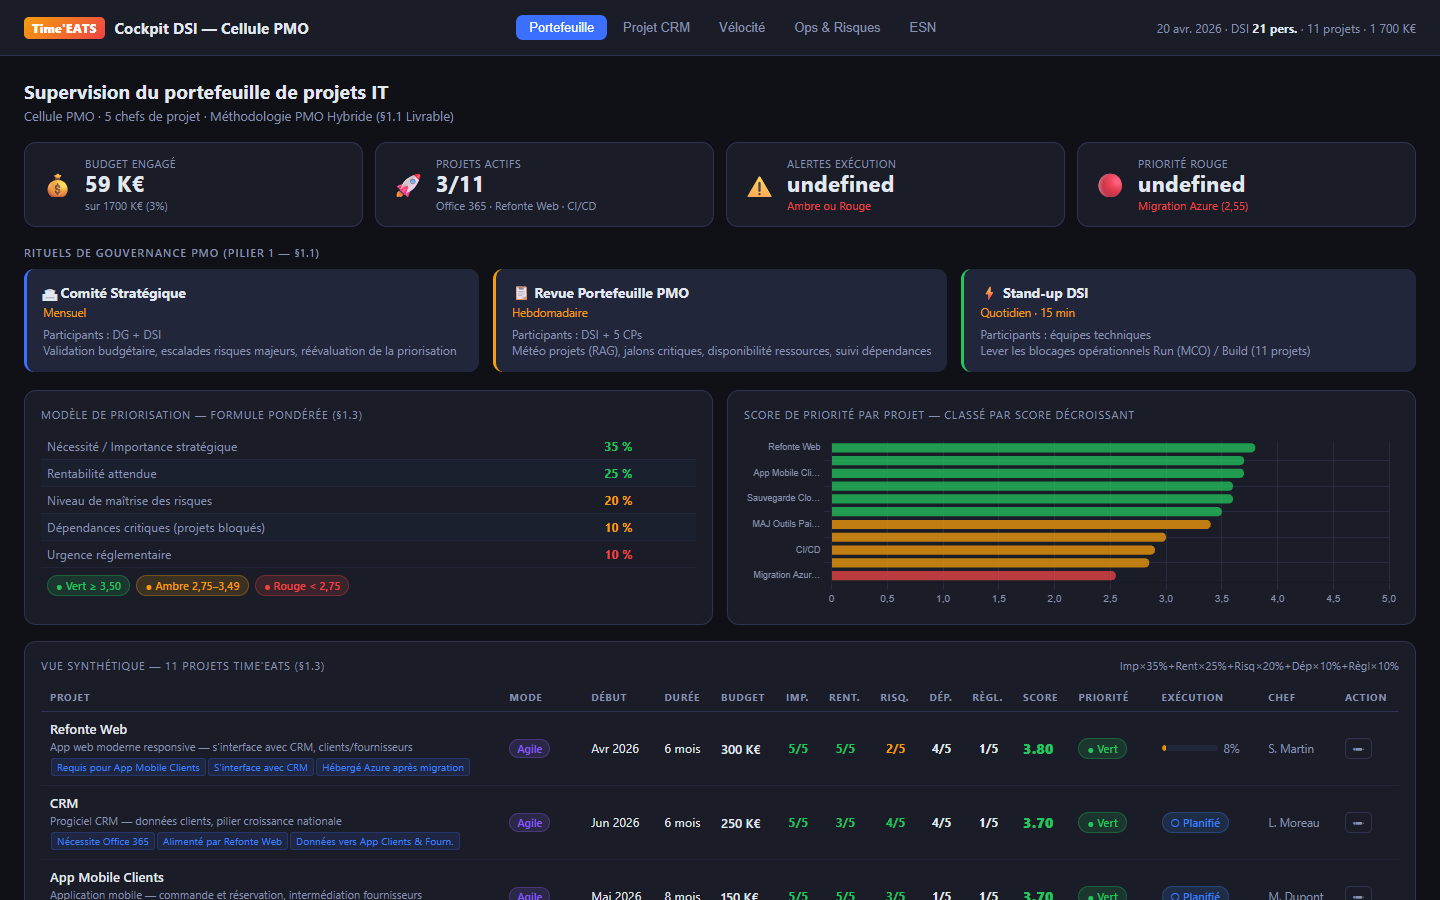
\includegraphics[width=\textwidth,keepaspectratio]{cockpit_portefeuille.png}
  \par\vspace{4pt}
  {\small\textcolor{cnSlate}{\textit{Capture — Onglet Portefeuille : supervision des 11 projets, score de priorisation, RAG exécution (Cockpit DSI — Avr 2026)}}}
\end{center}

\newpage
% ────────────────────────────────────────────────────────────
\section{Référentiel des indicateurs de pilotage}

\begin{finding}
Ce référentiel constitue la \textbf{liste exhaustive et consolidée} de tous les indicateurs mis en place dans le cadre PMO Time'Eats. Il couvre quatre niveaux de lecture : la supervision du portefeuille (vision DSI), le pilotage de projet (vision chef de projet), la performance PMO (vision amélioration continue) et les indicateurs opérationnels (vision infrastructure). Chaque indicateur est rattaché à son onglet source dans le Cockpit DSI.
\end{finding}

\subsection{Indicateurs de supervision du portefeuille}

Ces indicateurs alimentent l'\textbf{onglet Portefeuille} du Cockpit DSI via \texttt{GET /api/projects} et \texttt{GET /api/stats}.

\vspace{4pt}
\begin{center}
\renewcommand{\arraystretch}{1.5}
\begin{tabularx}{\textwidth}{L{4.5cm} L{3.5cm} C{2cm} C{2cm} L{2cm}}
\toprule
\rowcolor{cnNavy}
\th{Indicateur} & \th{Définition} & \th{Cible} & \th{Seuil alerte} & \th{Fréquence} \\
\midrule
Score de priorisation & $\sum$ (critère $\times$ poids) sur 5 axes & $\geq 3{,}50$ (Vert) & $< 2{,}75$ (Rouge) & Statique \\
\rowcolor{cnIce}
Statut RAG exécution & Rouge / Ambre / Vert sur Coûts + Délais + Qualité & Vert & Rouge & Mensuel \\
Avancement physique & \% de réalisation déclaré par le CP & Selon jalon & Retard $>10\,j$ & Mensuel \\
\rowcolor{cnIce}
Budget consommé / Budget prévu & Taux d'engagement budgétaire & $\leq 100\,\%$ & $> 110\,\%$ & Mensuel \\
Nombre de projets en alerte & Nb de projets en statut Ambre ou Rouge & 0 Rouge & $\geq 2$ Rouge & Hebdomadaire \\
\rowcolor{cnIce}
Dépendances critiques actives & Nb de projets bloqués par un prérequis non livré & 0 & $\geq 1$ bloquant & Hebdomadaire \\
Budget total engagé (portefeuille) & Somme des budgets consommés sur 11 projets & $\leq 1\,700$\,K€ & $>1\,785$\,K€ & Mensuel \\
\bottomrule
\end{tabularx}
\end{center}

\subsection{Indicateurs de pilotage projet (CRM — généralisable)}

Ces indicateurs alimentent l'\textbf{onglet Projet CRM} du Cockpit DSI via \texttt{GET /api/crm}. Ils sont applicables à tout projet du portefeuille disposant d'un PMP complet.

\vspace{4pt}
\begin{center}
\renewcommand{\arraystretch}{1.5}
\begin{tabularx}{\textwidth}{C{1.5cm} L{4cm} L{3.5cm} C{2cm} C{2cm} L{1.5cm}}
\toprule
\rowcolor{cnNavy}
\th{Axe} & \th{Indicateur} & \th{Calcul / Source} & \th{Cible} & \th{Seuil alerte} & \th{Fréq.} \\
\midrule
\multirow{3}{*}{\textbf{Coûts}} & Budget consommé / prévu & Comptabilité & $\leq 100\,\%$ & $> 110\,\%$ & Mensuel \\
\rowcolor{cnIce}
& IPC (Valeur acquise) & $\mathrm{VA} / \mathrm{CR}$ (EVM) & $\geq 0{,}9$ & $< 0{,}8$ & Mensuel \\
& Réserve pour aléas restante & Budget initial & $> 0\,\%$ & $< 5\,\%$ & Mensuel \\
\midrule
\rowcolor{cnIce}
\multirow{3}{*}{\textbf{Délais}} & Jalons respectés / planifiés & Planning & $= 100\,\%$ & $< 80\,\%$ & Mensuel \\
& IPD (Valeur acquise) & $\mathrm{VA} / \mathrm{VP}$ (EVM) & $\geq 0{,}9$ & $< 0{,}8$ & Mensuel \\
\rowcolor{cnIce}
& Retard cumulé (j. ouvrés) & Planning & 0 jour & $> 10\,j$ & Mensuel \\
\midrule
\multirow{3}{*}{\textbf{Qualité}} & Taux de couverture des tests & Log anomalies & $\geq 80\,\%$ & $< 60\,\%$ & Par sprint \\
\rowcolor{cnIce}
& Anomalies bloquantes ouvertes & Log anomalies & 0 & $> 2$ & Hebdom. \\
& Taux de satisfaction recette & Questionnaire métier & $\geq 85\,\%$ & $< 70\,\%$ & À la recette \\
\bottomrule
\end{tabularx}
\end{center}

\subsection{Indicateurs opérationnels (infrastructure et incidents)}

Ces indicateurs alimentent l'\textbf{onglet Ops \& Risques} du Cockpit DSI via \texttt{GET /api/servers} et \texttt{GET /api/incidents}.

\vspace{4pt}
\begin{center}
\renewcommand{\arraystretch}{1.5}
\begin{tabularx}{\textwidth}{L{4.5cm} L{4cm} C{2cm} C{2cm} L{2cm}}
\toprule
\rowcolor{cnNavy}
\th{Indicateur} & \th{Définition} & \th{Cible} & \th{Seuil alerte} & \th{Fréquence} \\
\midrule
Uptime moyen (9 serveurs) & \% disponibilité des serveurs on-premise & $\geq 99\,\%$ & $< 98\,\%$ & Temps réel \\
\rowcolor{cnIce}
Incidents P1 actifs & Incidents critiques (service arrêté) ouverts & 0 & $\geq 1$ & Temps réel \\
Incidents P2 actifs & Incidents majeurs (dégradation service) ouverts & 0 & $\geq 3$ & Quotidien \\
\rowcolor{cnIce}
Délai moyen résolution P1 & Délai entre ouverture et clôture d'un P1 & $\leq 5\,j$ & $> 5\,j$ & Par incident \\
Points bloquants ESN ouverts & Nb de blocages inter-équipes non levés & 0 & $\geq 2$ & Hebdomadaire \\
\rowcolor{cnIce}
Ancienneté dernier CR ESN & Nb de jours depuis le dernier compte-rendu & $\leq 14\,j$ & $> 30\,j$ & Mensuel \\
\bottomrule
\end{tabularx}
\end{center}

\subsection{Indicateurs de performance PMO (amélioration continue)}

Ces indicateurs alimentent la \textbf{section KPIs PMO} de l'onglet Ops \& Risques, calculés depuis les collections \texttt{projects} et \texttt{incidents}.

\vspace{4pt}
\begin{center}
\renewcommand{\arraystretch}{1.5}
\begin{tabularx}{\textwidth}{L{4.8cm} L{3.5cm} C{2cm} C{2cm} L{2cm}}
\toprule
\rowcolor{cnNavy}
\th{Indicateur PMO} & \th{Calcul} & \th{Cible} & \th{Valeur Avr N} & \th{Fréquence} \\
\midrule
\% projets dans les délais & Projets Vert délai / 11 & $\geq 80\,\%$ & n/d & Mensuel \\
\rowcolor{cnIce}
\% projets dans le budget & Projets Vert coût / 11 & $\geq 85\,\%$ & 100\,\% & Mensuel \\
Taux de satisfaction recette & Moyenne des questionnaires métier & $\geq 80\,\%$ & n/d & Par projet \\
\rowcolor{cnIce}
\% risques identifiés en amont & Risques préventifs / total risques & $\geq 70\,\%$ & 100\,\% & Semestriel \\
Taux de réutilisation templates & Projets utilisant le référentiel / 11 & $\geq 60\,\%$ & n/d & Semestriel \\
\rowcolor{cnIce}
Nb de REX produits & Fiches REX rédigées à la clôture & 1 / projet clos & 0 (phase init) & Par clôture \\
\bottomrule
\end{tabularx}
\end{center}

\begin{reco}
\textbf{Lecture croisée des indicateurs :} le Cockpit DSI est conçu pour que le DSI puisse passer de la vue macro (portefeuille, budget global) à la vue micro (KPIs d'un projet, détail d'un incident P1) en un seul clic. La cohérence entre les niveaux — supervision, pilotage, opérationnel, PMO — garantit qu'aucun signal faible ne passe entre les mailles.
\end{reco}

\newpage

% ============================================================
% CHAPITRE 2 — GESTION DU PROJET CRM
% ============================================================
\chapter{Gestion du projet : Progiciel CRM}

\begin{finding}
Le CRM est un progiciel destiné à centraliser les données clients existantes et à venir. Il constitue un \textbf{pilier stratégique} (importance 5/5) pour la mise en service des applications mobiles et de la Refonte Web. Démarrage : juin~N — Fin prévue : novembre~N — Budget : 250\,K€ — Charge : 300\,j/h.
\end{finding}

% ────────────────────────────────────────────────────────────
\section{Plan de management du projet CRM}

\subsection{Périmètre}

\textbf{Inclus :}
\begin{itemize}
  \item Sélection et déploiement d'un progiciel CRM marché (appel d'offres)
  \item Migration et nettoyage des données clients existantes (conformité RGPD)
  \item Intégration avec la Refonte Web (API REST) et le socle Office 365
  \item Paramétrage des profils utilisateurs (commerciaux, support, direction)
  \item Formation des utilisateurs clés et déploiement progressif
\end{itemize}
\textbf{Exclus :} développement spécifique sur le progiciel hors standard ; intégration apps mobiles (phase~2).

\subsection{Jalons clés}

\begin{center}
\renewcommand{\arraystretch}{1.5}
\begin{tabularx}{\textwidth}{C{2.2cm} L{5.5cm} C{2.8cm} L{3.5cm}}
\toprule
\rowcolor{cnNavy}
\th{Jalon} & \th{Description} & \th{Date cible} & \th{Critère d'entrée} \\
\midrule
J1 — Cadrage       & Validation note de cadrage + RACI             & 15 juin N  & Charte signée \\
\rowcolor{cnIce}
J2 — Sélection     & Choix de l'éditeur CRM, contractualisation     & 30 juin N  & AO dépouillé \\
J3 — Paramétrage   & Livraison environnement de recette             & 31 août N  & Contrat signé \\
\rowcolor{cnIce}
J4 — Recette       & Tests fonctionnels et validation métier        & 31 oct N   & Env. recette stable \\
J5 — Go-live       & Mise en production + formation utilisateurs    & 30 nov N   & PV recette signé \\
\bottomrule
\end{tabularx}
\end{center}

\subsection{WBS simplifié}

\begin{enumerate}
  \item \textbf{Cadrage et appel d'offres} (juin~N) : cahier des charges fonctionnel, publication et dépouillement de l'AO, choix de la solution
  \item \textbf{Paramétrage et intégration} (juillet–août~N) : installation, paramétrage des modules, développement des connecteurs API (Refonte Web), migration et nettoyage des données clients
  \item \textbf{Recette et formation} (septembre–octobre~N) : tests unitaires DSI, recette fonctionnelle métier, formation des Key Users
  \item \textbf{Déploiement et clôture} (novembre~N) : bascule en production, support post-ouverture J+30, clôture administrative
\end{enumerate}

\subsection{Budget prévisionnel}

\begin{center}
\renewcommand{\arraystretch}{1.5}
\begin{tabularx}{\textwidth}{L{5cm} R{2.5cm} R{2.5cm} L{3.8cm}}
\toprule
\rowcolor{cnNavy}
\th{Poste de dépense} & \th{Interne} & \th{ESN / Éditeur} & \th{Remarque} \\
\midrule
Licences CRM (1 an)        &         & 60\,K€  & Abonnement SaaS annuel \\
\rowcolor{cnIce}
Intégration / paramétrage  &         & 90\,K€  & Forfait ESN spécialisée \\
Migration des données       & 20\,K€ & 30\,K€  & Audit RGPD + nettoyage \\
\rowcolor{cnIce}
Formation utilisateurs      &  5\,K€ & 15\,K€  & Key Users + présentiel \\
Chef de projet (interne)    & 15\,K€ &         & 6 mois à 20\,\% charge \\
\rowcolor{cnIce}
Réserve pour aléas (10\,\%) &       & 15\,K€  & Déclenchée sur décision CP \\
\midrule
\rowcolor{cnNavy!15}
\textbf{Total}              & \textbf{40\,K€} & \textbf{210\,K€} & \textbf{250\,K€} \\
\bottomrule
\end{tabularx}
\end{center}

\subsection{Registre des risques}

\begin{center}
\renewcommand{\arraystretch}{1.5}
\scriptsize
\begin{tabularx}{\textwidth}{L{3.5cm} C{1.5cm} C{1.5cm} C{1.8cm} L{5.5cm}}
\toprule
\rowcolor{cnNavy}
\th{Risque} & \th{Proba.} & \th{Impact} & \th{Criticité} & \th{Plan de mitigation} \\
\midrule
Retard de l'éditeur CRM & Moyenne & Élevé & \cellcolor{cnOrange!30}\textbf{Majeur} & Contractualiser SLA avec pénalités ; jalons intermédiaires contractuels \\
\rowcolor{cnIce}
Données non conformes RGPD & Élevée & Élevé & \cellcolor{cnRed!30}\textbf{Critique} & Audit de données dès juin~N ; DPO impliqué au démarrage \\
Office 365 non terminé & Faible & Moyen & \cellcolor{cnGreen!30}\textbf{Mineur} & Planning conditionnel ; CRM peut démarrer en mode dégradé \\
\rowcolor{cnIce}
Résistance au changement & Moyenne & Moyen & \cellcolor{cnOrange!30}\textbf{Majeur} & Plan conduite du changement ; Key Users impliqués dès le cadrage \\
Dépassement budgétaire & Faible & Élevé & \cellcolor{cnOrange!30}\textbf{Majeur} & Jalons de validation budget (J2, J3, J4) ; réserve de 10\,\% \\
\rowcolor{cnIce}
Perte de données migration & Faible & Critique & \cellcolor{cnOrange!30}\textbf{Majeur} & Sauvegarde avant migration ; tests de non-régression \\
\bottomrule
\end{tabularx}
\end{center}
\normalsize

\subsection{Plan de communication}

\begin{center}
\renewcommand{\arraystretch}{1.5}
\begin{tabularx}{\textwidth}{L{4cm} L{3.5cm} C{2.2cm} C{2cm} L{2.8cm}}
\toprule
\rowcolor{cnNavy}
\th{Communication} & \th{Destinataires} & \th{Fréquence} & \th{Canal} & \th{Responsable} \\
\midrule
Réunion équipe projet & Équipe DSI + ESN & Hebdomadaire & Teams & Chef de projet \\
\rowcolor{cnIce}
Rapport d'avancement & DSI, DG & Mensuel & Email + SharePoint & Chef de projet \\
Comité de pilotage & DSI, DG, ESN & Mensuel & Présentiel & PMO \\
\rowcolor{cnIce}
Alerte critique & DSI, DG & Immédiat & Email + appel & Chef de projet \\
Newsletter utilisateurs & Commerciaux, support & Bi-mensuel & Email & CP + RH \\
\bottomrule
\end{tabularx}
\end{center}

% ────────────────────────────────────────────────────────────
\section{Tableau de bord de pilotage du projet CRM}

\begin{finding}
Ce tableau de bord est produit \textbf{mensuellement} par le chef de projet et présenté en COPIL. Le statut RAG permet une lecture immédiate de la santé du projet sur trois axes : Coûts, Délais, Qualité.
\end{finding}

\subsection{Indicateurs clés de performance}

\begin{center}
\renewcommand{\arraystretch}{1.5}
\begin{tabularx}{\textwidth}{L{2.8cm} L{4.5cm} C{2cm} C{2.2cm} L{3cm}}
\toprule
\rowcolor{cnNavy}
\th{Axe} & \th{Indicateur} & \th{Cible} & \th{Seuil alerte} & \th{Source} \\
\midrule
\multirow{3}{*}{\textbf{Coûts}} & Budget consommé / Budget prévu & $\leq 100\,\%$ & $>110\,\%$ & Comptabilité \\
\rowcolor{cnIce}
& IPC — Indice Performance Coût & $\geq 0{,}9$ & $<0{,}8$ & EVM \\
& Réserve pour aléas restante & $> 0\,\%$ & $< 5\,\%$ & Budget \\
\midrule
\rowcolor{cnIce}
\multirow{3}{*}{\textbf{Délais}} & Jalons respectés / Planifiés & $= 100\,\%$ & $< 80\,\%$ & Planning \\
& IPD — Indice Performance Délai & $\geq 0{,}9$ & $< 0{,}8$ & EVM \\
\rowcolor{cnIce}
& Retard cumulé (jours ouvrés) & 0 & $> 10\,j$ & Planning \\
\midrule
\multirow{3}{*}{\textbf{Qualité}} & Taux couverture des tests & $\geq 80\,\%$ & $< 60\,\%$ & Log anomalies \\
\rowcolor{cnIce}
& Anomalies bloquantes ouvertes & 0 & $> 2$ & Log anomalies \\
& Taux satisfaction recette & $\geq 85\,\%$ & $< 70\,\%$ & Questionnaire \\
\bottomrule
\end{tabularx}
\end{center}

\subsection{Fiche mensuelle de pilotage — Template papier}

Ce template est la \textbf{version papier} de la fiche mensuelle. La version live est alimentée en continu via l'onglet \og Projet CRM\fg{} du Cockpit DSI (cf. §1.3.4 et §2.3 ci-après).

\begin{center}
\renewcommand{\arraystretch}{1.5}
\begin{tabularx}{\textwidth}{L{3.2cm} C{1.8cm} C{1.8cm} C{1.8cm} L{5.5cm}}
\toprule
\rowcolor{cnNavy}
\th{KPI} & \th{Valeur M-1} & \th{Valeur M} & \th{Statut} & \th{Commentaire / Action} \\
\midrule
Budget consommé & — & — & \ragV & \\
\rowcolor{cnIce}
IPC (Coût)      & — & — & \ragV & \\
IPD (Délai)     & — & — & \ragA & \\
\rowcolor{cnIce}
Jalons respectés & — & — & \ragV & \\
Retard cumulé   & — & — & \ragV & \\
\rowcolor{cnIce}
Anomalies bloquantes & — & — & \ragV & \\
Taux couverture tests & — & — & \ragV & \\
\rowcolor{cnIce}
Satisfaction recette & — & — & \ragV & \\
\midrule
\rowcolor{cnNavy!15}
\multicolumn{5}{l}{\textbf{\textcolor{cnNavy}{Statut global du projet :}} \ragV} \\
\midrule
\multicolumn{5}{l}{\textbf{Points de vigilance du mois :}} \\
\multicolumn{5}{L{15cm}}{\itshape [3 points maximum — cf. registre des risques]} \\[2pt]
\multicolumn{5}{l}{\textbf{Décisions demandées au COPIL :}} \\
\multicolumn{5}{L{15cm}}{\itshape [Lister les décisions à prendre]} \\
\bottomrule
\end{tabularx}
\end{center}

% ────────────────────────────────────────────────────────────
\subsection{Intégration au Cockpit DSI — Onglet Projet CRM}

\begin{finding}
Le tableau de bord de pilotage CRM est opérationnellement géré via l'\textbf{onglet Projet CRM} du Cockpit DSI. Toutes les données présentées ci-dessus (KPIs, jalons, risques, vigilance COPIL) sont stockées dans la collection \texttt{crm\_kpis} de \texttt{db.json} et accessibles via \texttt{GET /api/crm}. La mise à jour se fait par \texttt{PATCH /api/crm/:id}.
\end{finding}

\textbf{Modèle de données CRM (\texttt{crm\_kpis} dans \texttt{db.json})}

\vspace{4pt}
\begin{center}
\renewcommand{\arraystretch}{1.5}
\begin{tabularx}{\textwidth}{L{3.8cm} L{2.5cm} L{7.5cm}}
\toprule
\rowcolor{cnNavy}
\th{Champ JSON} & \th{Type} & \th{Rôle} \\
\midrule
\texttt{kpis} & objet & 9 indicateurs : \texttt{budget\_pct}, \texttt{ipc}, \texttt{ipd}, \texttt{reserve\_pct}, \texttt{jalons\_pct}, \texttt{retard\_j}, \texttt{couverture\_tests}, \texttt{anomalies\_bloquantes}, \texttt{satisfaction\_pct} \\
\rowcolor{cnIce}
\texttt{jalons} & tableau & 5 jalons J1→J5 avec \texttt{id}, \texttt{desc}, \texttt{date\_cible}, \texttt{statut} (À venir / En cours / Terminé / Retard) \\
\texttt{statut\_global} & string & RAG consolidé automatiquement : \texttt{vert} / \texttt{ambre} / \texttt{rouge} \\
\rowcolor{cnIce}
\texttt{points\_vigilance} & tableau & Liste des points de vigilance présentés en COPIL (3 maximum) \\
\texttt{decisions\_copil} & tableau & Décisions à prendre par la direction lors du prochain COPIL \\
\rowcolor{cnIce}
\texttt{risques} & tableau & Registre des risques : \texttt{risque}, \texttt{proba}, \texttt{impact}, \texttt{criticite}, \texttt{mitigation} \\
\bottomrule
\end{tabularx}
\end{center}

\textbf{État initial du projet CRM au démarrage (Avr 2026 — phase pré-projet)}

\vspace{4pt}
\begin{center}
\renewcommand{\arraystretch}{1.5}
\begin{tabularx}{\textwidth}{L{4.5cm} C{2.5cm} L{7cm}}
\toprule
\rowcolor{cnNavy}
\th{KPI} & \th{Valeur actuelle} & \th{Commentaire} \\
\midrule
Budget consommé / prévu & — & Projet non démarré (Jun N) — réserve à 100\,\% \\
\rowcolor{cnIce}
IPC / IPD & — & Calcul EVM disponible dès J2 (contractualisation) \\
Anomalies bloquantes & 0 & Aucune anomalie ouverte \\
\rowcolor{cnIce}
Statut global & \ragV & Vert — aucun dépassement à ce stade \\
\bottomrule
\end{tabularx}
\end{center}

\begin{alert}
\textbf{3 points de vigilance actifs} dans le cockpit au démarrage : (1) décision progiciel CRM non finalisée — arbitrage Salesforce vs HubSpot ; (2) RFP CGI — réponse attendue avant le 30 avril ; (3) prérequis Office~365 à valider avant démarrage CRM. Ces points sont visibles en temps réel dans l'onglet \og Projet CRM\fg{} du Cockpit DSI.
\end{alert}

\vspace{6pt}
\begin{center}
  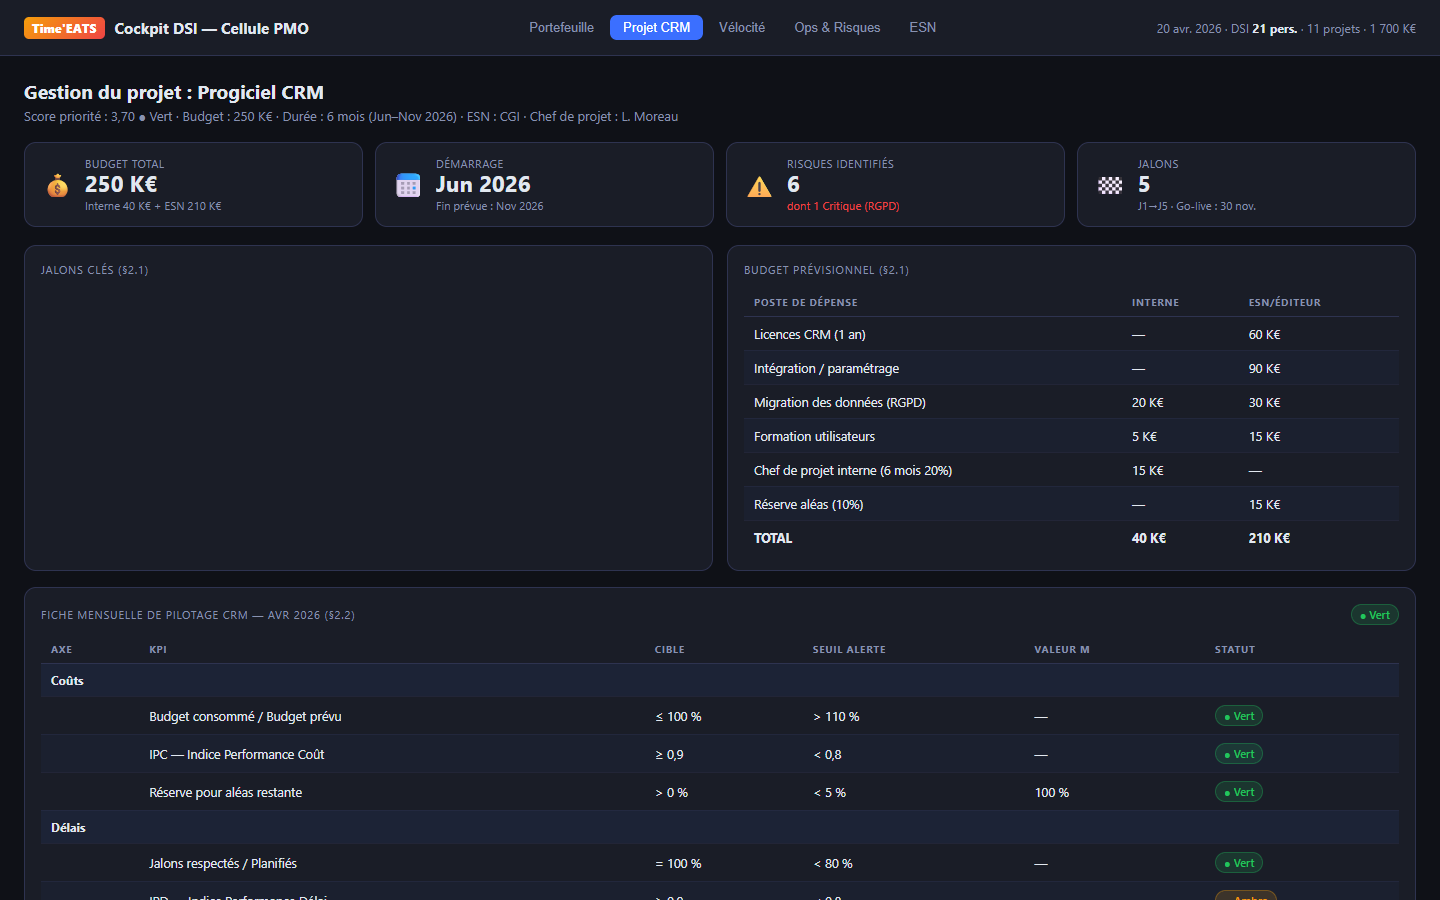
\includegraphics[width=\textwidth,keepaspectratio]{cockpit_crm.png}
  \par\vspace{4pt}
  {\small\textcolor{cnSlate}{\textit{Capture — Onglet Projet CRM : jalons J1→J5, KPIs mensuels RAG, registre des risques et vigilance COPIL (Cockpit DSI — Avr 2026)}}}
\end{center}

\newpage

% ============================================================
% CHAPITRE 3 — CLÔTURE ET CAPITALISATION
% ============================================================
\chapter{Clôture de projet et retour d'expérience}

% ────────────────────────────────────────────────────────────
\section{Documents contractuels de clôture du projet CRM}

\begin{reco}
La clôture ne se limite pas à la mise en production. Elle requiert un ensemble de documents formels qui \textbf{protègent juridiquement} l'entreprise, \textbf{libèrent les prestataires} et \textbf{transfèrent la responsabilité} au run. Chaque document est daté et signé.
\end{reco}

\subsection{Liste justifiée des documents de clôture}

\begin{center}
\renewcommand{\arraystretch}{1.5}
\begin{tabularx}{\textwidth}{C{0.5cm} L{4cm} L{4.5cm} L{4.5cm}}
\toprule
\rowcolor{cnNavy}
\th{\#} & \th{Document} & \th{Objectif} & \th{Signataires} \\
\midrule
1 & PV de recette fonctionnelle & Valider que le CRM répond aux exigences métier & CP + Représentants métier \\
\rowcolor{cnIce}
2 & PV de recette technique & Valider la conformité technique (perf., sécurité, intégration API) & CP + DSI Ops \\
3 & Rapport de clôture de projet & Bilan formel périmètre / coût / délai & CP + DSI \\
\rowcolor{cnIce}
4 & PV de transfert en exploitation & Remise officielle du système au run & CP + Responsable Ops \\
5 & Lettre de fin de mission ESN & Libérer contractuellement le prestataire & DSI + ESN \\
\rowcolor{cnIce}
6 & Bilan de conformité RGPD & Attester la conformité des données CRM & CP + DPO \\
7 & Dossier d'exploitation livré & Documentation technique pour le run (MCO) & CP + Lead Developer \\
\bottomrule
\end{tabularx}
\end{center}

\vspace{4pt}
\textbf{Justifications :}
\begin{itemize}
  \item Le \textbf{PV de recette fonctionnelle} est le déclencheur du paiement final à l'ESN — sans signature métier, aucun solde n'est versé.
  \item Le \textbf{PV de recette technique} couvre les risques d'intégration (API Refonte Web, connecteurs O365) et de performance sous charge.
  \item Le \textbf{PV de transfert} protège le chef de projet : toute anomalie post-transfert relève du run, pas du projet.
  \item La \textbf{lettre de fin de mission} est un acte juridique nécessaire pour clôturer les engagements contractuels.
  \item Le \textbf{bilan RGPD} est obligatoire pour tout système traitant des données personnelles (CNIL).
\end{itemize}

\newpage
\subsection{Template — Procès-verbal de recette fonctionnelle}

\begin{tcolorbox}[
  enhanced, colback=cnLightBlue, colframe=cnNavy,
  leftrule=4pt, rightrule=0pt, toprule=0.4pt, bottomrule=0.4pt,
  arc=0pt, boxsep=6pt, top=8pt, bottom=8pt, left=8pt, right=8pt
]
{\large\bfseries\textcolor{cnNavy}{PROCÈS-VERBAL DE RECETTE FONCTIONNELLE}}\\[2pt]
{\normalsize\textcolor{cnNavy}{Projet : Progiciel CRM — Time'Eats}}
\tcblower
\renewcommand{\arraystretch}{1.4}
\begin{tabularx}{\linewidth}{L{3.5cm} X L{3.5cm} X}
\textbf{Projet :} & CRM & \textbf{Version :} & 1.0 \\
\textbf{Date de recette :} & \rule{2.5cm}{0.4pt} & \textbf{Environnement :} & Production \\
\textbf{Chef de projet :} & \rule{2.5cm}{0.4pt} & \textbf{Éditeur CRM :} & \rule{2.5cm}{0.4pt} \\
\end{tabularx}

\vspace{6pt}
\textbf{\textcolor{cnNavy}{1. Périmètre testé}}
\vspace{4pt}

\begin{tabularx}{\linewidth}{C{0.5cm} L{5cm} C{2.5cm} C{2.5cm} L{3.5cm}}
\toprule
\rowcolor{cnNavy!20}
\textbf{\#} & \textbf{Fonctionnalité} & \textbf{Résultat} & \textbf{Statut} & \textbf{Réserves} \\
\midrule
1 & Gestion des contacts clients & Conforme & \cellcolor{cnGreen!25}OK & — \\
\rowcolor{cnIce}
2 & Gestion des opportunités commerciales & Conforme & \cellcolor{cnGreen!25}OK & — \\
3 & Import des données clients & À contrôler & \cellcolor{cnOrange!25}À valider & Vérifier doublons \\
\rowcolor{cnIce}
4 & Intégration API Refonte Web & Conforme & \cellcolor{cnGreen!25}OK & — \\
5 & Rapports et tableaux de bord CRM & Conforme & \cellcolor{cnGreen!25}OK & — \\
\rowcolor{cnIce}
6 & Gestion des accès et profils & Conforme & \cellcolor{cnGreen!25}OK & — \\
\bottomrule
\end{tabularx}

\vspace{6pt}
\textbf{\textcolor{cnNavy}{2. Critères d'acceptance}}
\begin{itemize}
  \item Toutes les fonctionnalités du périmètre livrées et testées
  \item 0 anomalie bloquante (P1) ouverte à la date de signature
  \item Taux de satisfaction utilisateurs lors des tests $\geq 80\,\%$
  \item Documentation utilisateur livrée et validée
\end{itemize}

\vspace{6pt}
\textbf{\textcolor{cnNavy}{3. Résultat global}}
\vspace{4pt}

\begin{tabularx}{\linewidth}{L{7cm} C{3cm}}
Cas de test exécutés : & \rule{3cm}{0.4pt} \\
Cas OK : & \rule{3cm}{0.4pt} \\
Anomalies bloquantes : & \rule{3cm}{0.4pt} \\
Anomalies mineures : & \rule{3cm}{0.4pt} \\
\end{tabularx}

\vspace{6pt}
\textbf{\textcolor{cnNavy}{4. Décision}}
\vspace{4pt}

\begin{tabularx}{\linewidth}{C{4cm} C{4cm} C{4cm}}
\cellcolor{cnGreen!25}\textbf{Recette acceptée} & \cellcolor{cnOrange!25}\textbf{Acceptée avec réserves} & \cellcolor{cnRed!25}\textbf{Recette refusée} \\
$\square$ & $\square$ & $\square$ \\
\end{tabularx}

\vspace{6pt}
\textbf{\textcolor{cnNavy}{5. Réserves et plan de levée}}\\[8pt]
\rule{\linewidth}{0.4pt}\\[12pt]
\textbf{\textcolor{cnNavy}{6. Signatures}}

\begin{tabularx}{\linewidth}{X X X}
\textbf{Chef de projet} & \textbf{Représentant Métier} & \textbf{DSI} \\[14pt]
\rule{4cm}{0.4pt} & \rule{4cm}{0.4pt} & \rule{4cm}{0.4pt} \\
Date : \rule{1.8cm}{0.4pt} & Date : \rule{1.8cm}{0.4pt} & Date : \rule{1.8cm}{0.4pt} \\
\end{tabularx}
\end{tcolorbox}

\newpage
% ────────────────────────────────────────────────────────────
\section{Capitalisation et amélioration continue}

\subsection{Enjeux pour Time'Eats}

La DSI pilote 11 projets avec 5 chefs de projet. Sans capitalisation structurée, chaque erreur sera répétée et chaque bonne pratique perdue. L'amélioration continue est un \textbf{levier de productivité immédiat} — et sa mise en œuvre ne requiert aucun budget supplémentaire.

\subsection{Processus de capitalisation — 4 étapes}

\begin{center}
\renewcommand{\arraystretch}{1.5}
\begin{tabularx}{\textwidth}{C{1cm} L{3.8cm} L{5.5cm} L{3.5cm}}
\toprule
\rowcolor{cnNavy}
\th{Étape} & \th{Activité} & \th{Description} & \th{Outil} \\
\midrule
1 & Rétrospective de clôture & Séance 2h avec l'équipe : ce qui a fonctionné, ce qui a posé problème, 3 actions d'amélioration & Teams / Miro \\
\rowcolor{cnIce}
2 & Rédaction fiche REX & Synthèse structurée : contexte, enseignements, recommandations, fichiers liés & SharePoint O365 \\
3 & Mise à jour du référentiel & Templates concernés mis à jour, bonnes pratiques PMO enrichies & SharePoint O365 \\
\rowcolor{cnIce}
4 & Revue semestrielle PMO & Analyse des REX accumulés, patterns récurrents, mise à jour du référentiel & COPIL semestriel \\
\bottomrule
\end{tabularx}
\end{center}

\subsection{Boucle PDCA appliquée au PMO}

\begin{itemize}
  \item \textbf{Plan} : Définir les processus PMO et les templates du référentiel (effectué au démarrage PMO)
  \item \textbf{Do} : Appliquer le référentiel sur chaque projet du portefeuille
  \item \textbf{Check} : Collecter les REX à la clôture ; mesurer les indicateurs PMO (respect budgétaire, taux de jalons, satisfaction métier)
  \item \textbf{Act} : Mettre à jour le référentiel sur la base des enseignements ; présenter au COPIL semestriel
\end{itemize}

\subsection{Indicateurs de performance du PMO}

Ces indicateurs sont \textbf{centralisés dans l'onglet Ops \& Risques du Cockpit DSI} — section \og Indicateurs de performance PMO\fg{}. Ils sont mis à jour automatiquement à partir des données de la collection \texttt{projects} (avancement, budget consommé) et de la collection \texttt{incidents} (délai de résolution P1).

\begin{center}
\renewcommand{\arraystretch}{1.5}
\begin{tabularx}{\textwidth}{L{5cm} C{3cm} C{2cm} L{4cm}}
\toprule
\rowcolor{cnNavy}
\th{Indicateur PMO} & \th{Cible} & \th{Valeur Avr N} & \th{Source Cockpit} \\
\midrule
\% projets dans les délais & $\geq 80\,\%$ & n/d & \texttt{/api/projects} \\
\rowcolor{cnIce}
\% projets dans le budget & $\geq 85\,\%$ & 100\,\% & \texttt{/api/stats} \\
Taux satisfaction à la recette & $\geq 80\,\%$ & n/d & \texttt{/api/crm} \\
\rowcolor{cnIce}
\% risques identifiés en amont & $\geq 70\,\%$ & 100\,\% & \texttt{/api/projects} \\
Délai moyen résolution P1 & $\leq 5\,j$ & 3\,j & \texttt{/api/incidents} \\
\rowcolor{cnIce}
Taux de réutilisation des templates & $\geq 60\,\%$ & n/d & Manuel (REX) \\
\bottomrule
\end{tabularx}
\end{center}

\begin{reco}
Cette démarche ne représente \textbf{aucun coût additionnel} : le Cockpit DSI s'appuie sur Node.js (runtime gratuit) et SharePoint Online (déjà financé par le projet Office~365) pour le stockage des REX et des templates. Le ROI est direct : une heure de rétrospective bien menée évite de répéter les mêmes erreurs sur les 11 projets restants.
\end{reco}

\vspace{6pt}
\begin{center}
  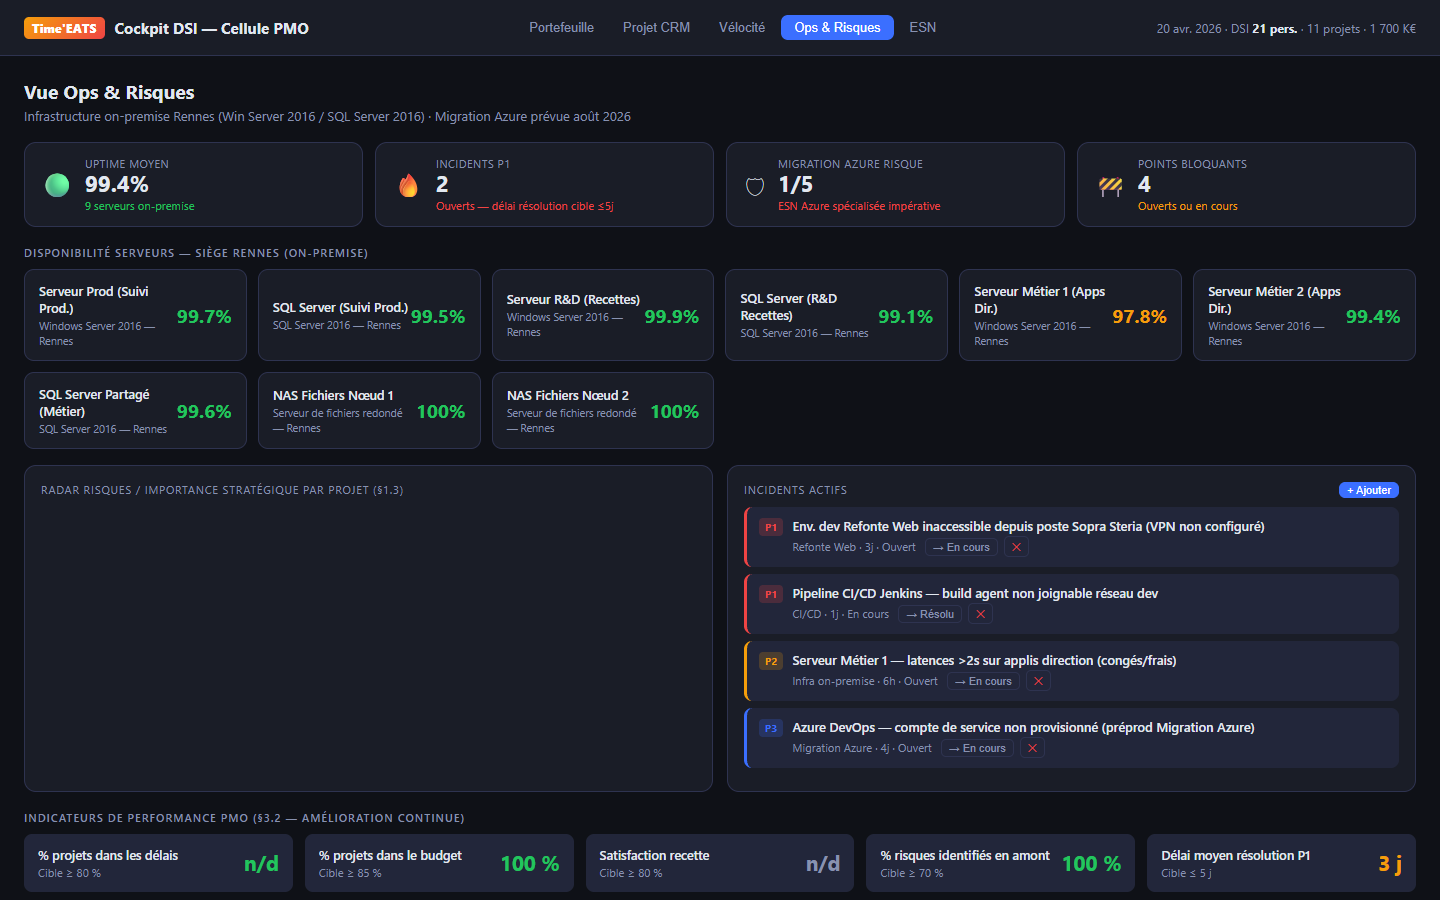
\includegraphics[width=\textwidth,keepaspectratio]{cockpit_ops.png}
  \par\vspace{4pt}
  {\small\textcolor{cnSlate}{\textit{Capture — Onglet Ops \& Risques : uptime serveurs, incidents P1/P2/P3, KPIs PMO (Cockpit DSI — Avr 2026)}}}
\end{center}

\vspace{6pt}
\begin{center}
  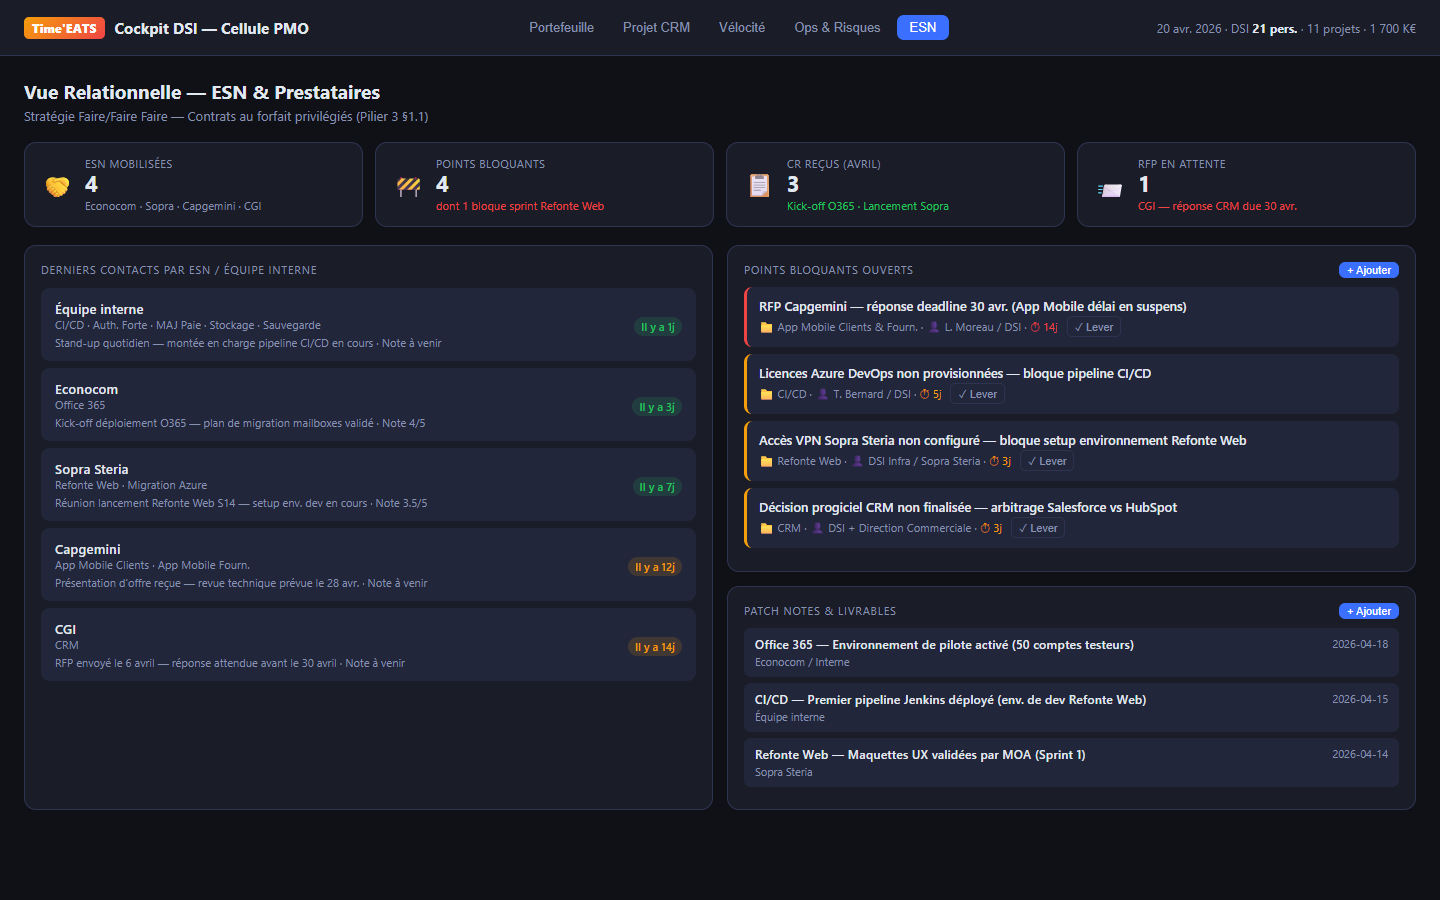
\includegraphics[width=\textwidth,keepaspectratio]{cockpit_esn.png}
  \par\vspace{4pt}
  {\small\textcolor{cnSlate}{\textit{Capture — Onglet ESN : suivi des contacts, points bloquants, livrables ESN (Cockpit DSI — Avr 2026)}}}
\end{center}

\newpage

% ── Annexe checklist ─────────────────────────────────────────
\chapter*{Annexe — Checklist grille d'évaluation}
\addcontentsline{toc}{chapter}{Annexe — Checklist grille d'évaluation}

\begin{center}
\renewcommand{\arraystretch}{1.6}
\begin{tabularx}{\textwidth}{C{0.5cm} L{7cm} C{2cm} C{1.8cm} C{3cm}}
\toprule
\rowcolor{cnNavy}
\th{\#} & \th{Critère de la grille} & \th{Points} & \th{Couvert} & \th{Référence} \\
\midrule
\multicolumn{5}{l}{\cellcolor{cnNavy!15}\textbf{\textcolor{cnNavy}{Axe 1 — Définir, prioriser et faire vivre le portefeuille (8 pts)}}} \\
\midrule
1 & Processus de management basé sur standards & 2 pts & \cellcolor{cnGreen!25}Oui & §1.2 \\
\rowcolor{cnIce}
2 & Plan du référentiel documentaire & 3 pts & \cellcolor{cnGreen!25}Oui & §1.3 \\
3 & Template tableau de bord supervision & 3 pts & \cellcolor{cnGreen!25}Oui & §1.4 \\
\midrule
\multicolumn{5}{l}{\cellcolor{cnNavy!15}\textbf{\textcolor{cnNavy}{Axe 2 — Superviser et conduire les projets IT (5 pts)}}} \\
\midrule
\rowcolor{cnIce}
4 & Plan de management complet (CRM) & 3 pts & \cellcolor{cnGreen!25}Oui & §2.1 \\
5 & Tableau de bord de suivi projet & 2 pts & \cellcolor{cnGreen!25}Oui & §2.2 \\
\midrule
\multicolumn{5}{l}{\cellcolor{cnNavy!15}\textbf{\textcolor{cnNavy}{Axe 3 — Clore les projets et capitaliser (5 pts)}}} \\
\midrule
\rowcolor{cnIce}
6 & Documents contractuels de clôture & 2 pts & \cellcolor{cnGreen!25}Oui & §3.1 \\
7 & Processus d'amélioration continue & 3 pts & \cellcolor{cnGreen!25}Oui & §3.2 \\
\midrule
\rowcolor{cnNavy!15}
\textbf{} & \textbf{TOTAL} & \textbf{20 pts} & \textbf{\textcolor{cnGreen}{100\,\%}} & \\
\bottomrule
\end{tabularx}
\end{center}

\vfill
\begin{center}
\tiny\textcolor{cnSlate}{Document confidentiel — Cellule PMO — Time'Eats — CESI MAALSI 2026}
\end{center}

\end{document}
